\documentclass[12pt, letterpaper, titlepage]{article}

\usepackage{amsmath}
\usepackage{booktabs}
\usepackage{amsthm}
\usepackage{graphicx}
\usepackage[margin=1in]{geometry}
\usepackage{hyperref}
\hypersetup{colorlinks = true, linkcolor = blue, citecolor=blue, urlcolor = blue}
\usepackage{natbib}
\usepackage{enumitem}
\usepackage{setspace}

\usepackage[pagewise]{lineno}
%\linenumbers*[1]
% %% patches to make lineno work better with amsmath
\newcommand*\patchAmsMathEnvironmentForLineno[1]{%
 \expandafter\let\csname old#1\expandafter\endcsname\csname #1\endcsname
 \expandafter\let\csname oldend#1\expandafter\endcsname\csname end#1\endcsname
 \renewenvironment{#1}%
 {\linenomath\csname old#1\endcsname}%
 {\csname oldend#1\endcsname\endlinenomath}}%
\newcommand*\patchBothAmsMathEnvironmentsForLineno[1]{%
 \patchAmsMathEnvironmentForLineno{#1}%
 \patchAmsMathEnvironmentForLineno{#1*}}%

\AtBeginDocument{%
 \patchBothAmsMathEnvironmentsForLineno{equation}%
 \patchBothAmsMathEnvironmentsForLineno{align}%
 \patchBothAmsMathEnvironmentsForLineno{flalign}%
 \patchBothAmsMathEnvironmentsForLineno{alignat}%
 \patchBothAmsMathEnvironmentsForLineno{gather}%
 \patchBothAmsMathEnvironmentsForLineno{multline}%
}

% control floats
\renewcommand\floatpagefraction{.9}
\renewcommand\topfraction{.9}
\renewcommand\bottomfraction{.9}
\renewcommand\textfraction{.1}
\setcounter{totalnumber}{50}
\setcounter{topnumber}{50}
\setcounter{bottomnumber}{50}

\newcommand{\jy}[1]{\textcolor{blue}{JY: #1}}
\newcommand{\eds}[1]{\textcolor{red}{EDS: (#1)}}


\title{On Misuses of the Kolmogorov--Smirnov Test for One-Sample Goodness-of-Fit}

\author{Anthony Zeimbekakis\\
%   \href{mailto:anthony.zeimbekakis@uconn.edu}
% {\nolinkurl{anthony.zeimbekakis@uconn.edu}}\\
  Elizabeth Schifano\\
  Jun Yan\\[1ex]
  Department of Statistics, University of Connecticut\\
}
\date{}

\begin{document}
\maketitle

\doublespace

\begin{abstract}
The Kolmogorov--Smirnov (KS) test is one of the most popular goodness-of-fit
tests for comparing a sample with a hypothesized continuous distribution.
Nevertheless, it has often been misused. The standard one-sample KS test applies
to independent, continuous data with a hypothesized distribution that is
completely specified. It is not uncommon, however, to see in the literature that
it was applied to dependent, discrete, or rounded data, with hypothesized
distributions containing estimated parameters. For example, it has been
``discovered'' multiple times that the test is too conservative when
hypothesized distribution has parameters that need to be estimated.
We demonstrate misuses of the one-sample KS test in
three scenarios through simulation studies:
1) the hypothesized distribution has unspecified parameters;
2) the data are serially dependent; and
3) a combination of the first two scenarios.
For each scenario, we provide remedies for practical applications.

\bigskip
\noindent{\sc Keywords}:
nonparametric bootstrap;
parametric bootstrap.
\end{abstract}

\section{Introduction}
\label{sec:intro}

The Kolmogorov-Smirnov (KS) test is one of the most popular goodness-of-fit
tests for comparing a sample with a hypothesized parametric distribution.
Let $X_1, ..., X_n$ be a random sample of size~$n$ from a continuous
distribution. The null hypothesis $H_0$ is that $X_i$'s follow distribution~$F$.
Let $F_n(t) = \sum_{i=1}^n I(X_i \le t) / n$ be the empirical cumulative
distribution function of the sample, where $I(\cdot)$ is the indicator
function. The KS test statistic is
\begin{equation}
  \label{eq:ks_standard}
  D_n = \sup_x | F_{n}(x) - F(x) |.
\end{equation}
The asymptotic distribution of $D_n$ under $H_0$ is independent of the
distribution $F$. As $n \to \infty$, $\sqrt{n} D_n$ converges in distribution to
the supremum of standard Brownian bridge \citep{kolmogorov1933sulla}. For large
samples, the tests can be performed with a table \citep{smirnov1948table}.
Critical values for small samples ($n \le 35$) has also been given
\citep{Massey}. The KS test is available in popular
statistical software packages, such as function \texttt{ks.test} in R package
\textsf{stats} \citep{R, Marsaglia}.


The standard one-sample KS test applies to independent data with a continuous
hypothesized distribution that is completely specified. In practice, however, it
has often been applied without realizing that one or more of these assumptions
do not hold. For example, \citet{Noether} demonstrated the conservativeness of
the KS test when applied to discontinuous distributions. The null distribution
of the KS statistic is no longer distribution free. Computing the
exact and asymptotic distribution of $D_n$ is challenging. Fortunately, the null
distribution of the KS statistic when the underlying distribution is
discontinuous has been efficiently addressed by \citet{Dimitrova} with an
companion R package \textsf{KSgeneral}. Although a common misuse of KS test, the
issue with discontinuous or data is not our focus.


When the hypothesized distribution contains fitted parameters, as is the case in
most goodness-of-fit test settings, the standard KS test is not applicable.
\citet{Steinskog} ``discovers'' the change in power
when using fitted parameters and stresses caution in using the KS test in
such ways. In fact, using fitted parameters in place of the true parameters in
KS test is long known to yield extremely conservative results
\citep[e.g.,][]{Lilliefors}. This problem can be solved by parametric
bootstrap \citep{efron1985bootstrap, hall1991two}, where
bootstrap samples of the testing statistics are constructed from samples
generated from the fitted hypothesized distribution. A nonparametric bootstrap
solution is not trivial because the a nonparametric bootstrap sample of the
observed data have ties, which would not happen for continuous distributions.
\citet{Babu} derived the bias of standard nonparametric bootstrap and
showed how to correct it. They further noted that both parametric and
non-parametric procedures lead to correct asymptotic levels.


The standard KS test does not apply to serially dependent data either. The
distribution of the KS statistic would have a higher variance for positively
dependent data than that derived when the data are independent because of a
smaller effective sample size. For example, for
testing normality, \citet{Durilleul} demonstrates that a naive application of
the KS statistic is too liberal for medium-to-high positive serieal dependence,
and that for negative dependence, the behavior is asymmetrical. For remedies,
\citet{Weiss} provides a procedure that is applicable specifically for data
modeled by the second-order auto-regressive (AR) process where the AR parameters
are known. \citet{Lanzante} tests various strategies for dealing with temporal
dependence and concludes that a test based on Monte-Carlo simulations performed
the best. When additionally the hypothesized distribution contains unknown
parameters, the standard KS test becomes even further inapplicable.


The contribution of this paper is a demonstration of misuses of the one-sample
KS test in three scenarios and their remedies in practice. The scenarios are
where:
1) the hypothesized distribution has unspecified parameters;
2) the data are serially dependent; and
3) a combination of the first two scenarios.
In each scenario, the misuse is performed and the impacts are shown. Then, a
remedy is detailed and performed alongside the misuse to show its positive
effects. In order to set up the demonstrations, simulated data is used
throughout. The remedies are also performed on various families of
distributions.


The rest of the paper is organized as follows. Section~\ref{sec:fitted}
investigates the scenario where the hypothesized distribution has unspecified
parameters. Both parametric and nonparametric bootstrap are available to fix the
issue. Section~\ref{sec:dependence} investigates the scenario where the data of
the empirical distribution is serially dependent. A bootstrap procedure
employing copulas to account for dependence is proposed as a working solution.
Section~\ref{sec:fittedwithdependence}
explores the case where a combination of the first two scenarios occurs. The
copula procedure can be adjusted for the use of fitted parameters as a remedy.
Section~\ref{sec:conclusion} concludes with a discussion.

\section{Unspecified Parameters}
\label{sec:fitted}

The null distribution of the KS statistic changes when the hypothesized
distribution contains fitted parameters.
\eds{what is the null distribution when not using fitted parameters}.
In this scenario, the null hypothesis
is $H_0$: the random sample $X_1, \ldots, X_n$ comes from a continuous
distribution $F_{\theta}$ with unspecified parameter vector $\theta$.
Let $\hat\theta_n$ be an estimator of $\theta$, which could be, for example, a
maximum likelihood estimator or moment estimator. The test statistic is
\begin{equation}
  \label{eq:ks_fitted}
  D = \sup_x | F_n(x) - F_{\hat\theta_n}(x) |.
\end{equation}
Since $F_{\hat\theta_n}$ is not the same as the true data generating
$F_\theta$, the null distribution of $D$ obtained in existing implementations in
software packages which assumes completely known $F_\theta$ no longer applies
\citep{Steinskog}.


To demonstrate the consequences of this problem, a simulation is performed. A
random sample $X_1, \ldots, X_n$ is generated from the standard normal
distribution with sample size $n = 100$. The p-values of $1000$ replicate tests
 of normality
are displayed in the Naive plot of Figure~\ref{fig:hist_fitted}.
\eds{how are these p-values calculated?}
Each KS test
was performed using fitted parameters, i.e., the hypothesized distribution is
$N(\bar X, s^2)$ where $\bar X$ is the sample mean and $s^2$ is the sample
variance. Since the data is truly generated from a standard normal distribution,
 %with
%seemingly all assumptions met,
a uniform distribution of $U(0, 1)$ would naively be expected for the p-values.
However this should only be expected when the KS test assumptions hold, and they
 do not due to using fitted parameters. Therefore,
there is notable deviation from the uniform distribution.


To fix the problem, parametric bootstrap can be used to approximate the null
distribution of the testing statistic.
\begin{enumerate}
  \item
    Draw a random sample $X_1^*,...,X_n^*$ from the fitted distribution
    $F_{\hat\theta_n}$
  \item
    Fit $F_\theta$ to the sample and obtain estimated $\hat\theta_n^*$
  \item
    Obtain the empirical distribution function $F_n^*$ of $X_1^*, \ldots,
    X_n^*$.
  \item
    Calculate bootstrap KS statistic
    \[
      D^* = \sup_x | F_n^* (x)- F_{\hat\theta_n}^*(x) |.
    \]
  \item
    Repeat the previous steps a large number $B$ times and use the empirical
    distribution of $D^*$ to approximate the null distribution of the observed
    statistic.
\end{enumerate}


Nonparametric bootstrap can also be used to approximate the null distribution
of the testing statistic. The procedure is similar, however the resampling is
performed with the empirical distribution instead of the fitted parametric
distribution and there is a correction for bias that is required
\citep{Babu}.
\begin{enumerate}
  \item
    Draw a random sample $X_1^*,...,X_n^*$ from the empirical distribution $F_n$
    with replacement
  \item
    Fit $F_\theta$ to the sample and obtain estimated $\hat\theta_n^*$
  \item
    Obtain the empirical distribution function of the random sample $F_n^*$
  \item
    Calculate bootstrap KS statistic
    \[
      D^* = \sup_x | F_n^* (x)- F_{\hat\theta_n}^*(x) - B_n(x) |.
    \]
    where $B_{n}(x) = \sqrt{n}(F_{n}(x) - F_{\hat\theta_n}(x))$ is the known
    bias term \citep{Babu}
  \item
    Repeat the previous steps a large number $B$ times and use the empirical
    distribution of $D^*$ to approximate the null distribution of the observed
    statistic.
\end{enumerate}
The p-value can be calculated by counting the number of bootstrap KS
statistics greater than or equal to the observed KS statistic, and then dividing
by the number of bootstrap samples. Figure~\ref{fig:hist_fitted} displays the
results of from our simulations. We would expect the distribution of p-values
to be uniform in the case where the KS test holds its size. It is clear from the
figure that both parametric and nonparametric bootstrap processes correct for
the problem of fitted parameters. The plots for the bootstrapped p-values appear
to be $U(0,1)$, unlike the naive p-values.

\begin{figure}[tbp]
  \centering
  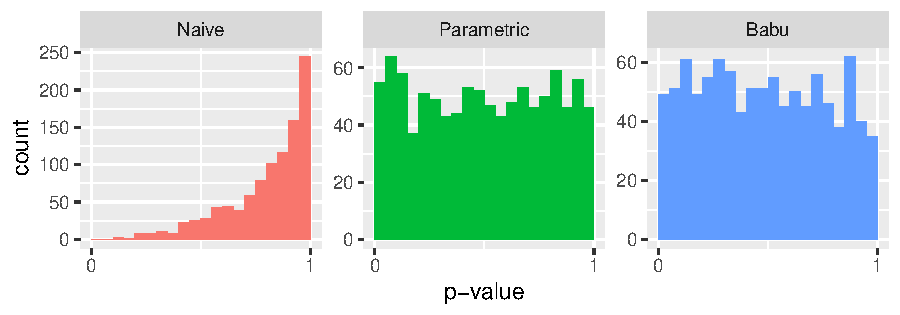
\includegraphics[width=\textwidth]{hist_fitted}
  \caption{The Naive plot (left) is the histogram of p-values from the standard
  KS test with fitted parameters. The Parametric plot (middle) is the histogram
  of p-values from implementing parametric bootstrap. The Babu plot (right) is
  the histogram of p-values from implementing nonparametric bootstrap with a
  correction for bias. In each case, $1000$ replicate tests were performed on
  the standard normal distribution with sample size $n = 100$. $B = 1000$
  bootstrap samples are obtained for each test. \eds{perhaps use density hist vs
	freq. hist (here and elsewhere)?}}
  \label{fig:hist_fitted}
\end{figure}


\section{Serially Dependent Data}
\label{sec:dependence}

The KS test also displays issues in the case of dependent data. As mentioned, an
assumption of the test is that the data is independent. Real data, however,
is often temporally or spatially dependent and the results of a goodness-of-fit
test would be valuable. When the KS test is performed on dependent data it
performs poorly. In this situation, the null hypothesis is $H_0$: the random
sample $X_1, \ldots, X_n$ come from a continuous distribution $F$ where $F$ has
completely specified parameters. The test statistic is the same as
Equation~\eqref{eq:ks_standard}. However, since the data is dependent, the null
hypothesis is wrong and must be corrected.
\eds{null hypothesis or null distribution? or both?}
This is demonstrated with a
simulation in Figure~\ref{fig:hist_correlation}. Data is generated from a
first-order autoregressive model (AR(1)) with a standard normal distribution.
P-values are gathered from $1000$ replicate tests for different levels of the
AR coefficient $\psi$, varying from $(-3,3)$.
\eds{how are these p-values calculated?}
In the presence of serially
dependent data, the distribution of p-values no longer follows $U(0, 1)$ as
would be expected of a valid test. The results echo those of \citet{Durilleul}
that the KS statistic is too liberal in the presence of positive
autocorrelation, and that the behavior is asymmetrical for negative
 autocorrelation.

\begin{figure}[tbp]
  \centering
  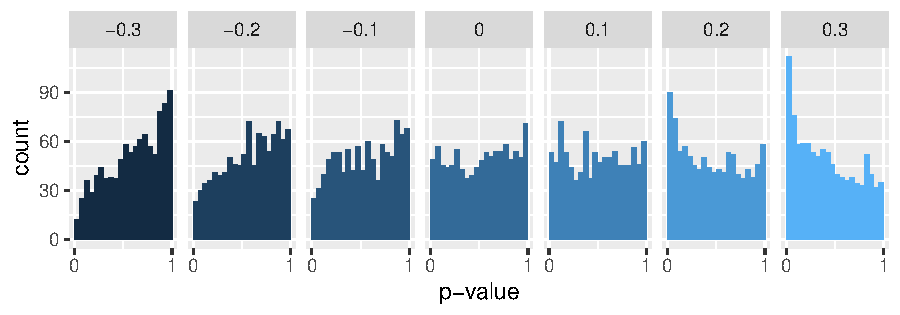
\includegraphics[width=\textwidth]{hist_correlation}
  \caption{Each histogram is a plot of the p-values of standard KS tests
  performed on dependent data simulated from an AR(1) process of the standard
  normal distribution. The titles represent the various levels of the AR
  coefficient $\psi$ tested. The sample size is $n = 100$ and $1000$ replicate
  tests were performed for each AR coefficient.}
  \label{fig:hist_correlation}
\end{figure}

In order to correct this, we can employ a parametric bootstrap procedure which
assumes a working serial dependence structure through copulas. A copula is a
multivariate distribution with standard uniform marginal distributions, which
completely characterizes the dependence structure of a multivariate
distribution \citep{Copula, Hofert}. For simplicity, we assume a normal copula
with an AR(1) structure to characterize the serial dependence of the
observations. The AR(1) parameter $r$ of the normal copula is set to match the
sample serial Spearman's rho of the observed data.
\eds{What is the difference between $\psi$ and $r$?}
The procedure is as
follows.

\begin{enumerate}
\item
  Generate $Z_1, \ldots, Z_n$ from an AR(1) process with autocorrelation
  coefficient $r$ such that the $Z_i$'s are $N(0, 1)$ variables.
\item
  Form a bootstrap sample $X_i^* = F^{-1} [\Phi(Z_i)]$, where $\Phi$ is the
  distribution function of $N(0, 1)$, $i = 1, \ldots, n$, whose first-order
  sample Spearman's rho matches that of the observed data.
\item
  Obtain the empirical distribution function $F_n^*$ of the bootstrap sample
  $X_1^*, \ldots, X_n^*$.
\item
  Calculate bootstrap KS statistic
  \[
    D^* = \sup_x \lvert F_n^* (x)- F(x) \rvert.
  \]
\item
  Repeat the previous steps a large number $B$ times and use the empirical
    distribution of the $B$ test statistics to approximate
    the null distribution of the observed statistic.
\end{enumerate}

Throughout the simulation we assume a working AR(1) dependence structure
regardless of the true dependence. If the true dependence is indeed a normal
copula with an AR(1) structure, this method is exact. When the true dependence
is not AR(1), it may still give a reasonable approximation that can be useful
for practical purposes. This is demonstrated with different dependence
structures in Figure~\ref{fig:hist_ma1_arma_ar2_D}.

\begin{figure}[tbp]
  \centering
  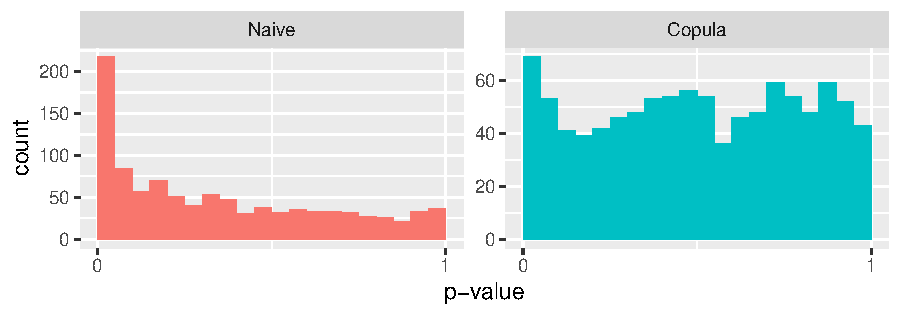
\includegraphics[width=\textwidth]{hist_ar1_D}
  \caption{The Naive plot (left) is the histogram of p-values from the
  standard KS test. The Copula plot (right) is the histogram of p-values from
  implementing parametric bootstrap with copulas for dependence. In each case,
  $1000$ replicate tests were performed with the data generated from an AR(1)
  process of the standard normal distribution with $\psi = .5$. The sample size
  is $n = 100$ and $B = 1000$ bootstrap samples are obtained for each test.}
  \label{fig:hist_ar1_D}
\end{figure}

Figure~\ref{fig:hist_ar1_D} displays the results of the copula remedy for
dependent data. The data is generated from the standard normal distribution with
an AR(1) dependence structure where $\psi = .5$. The copula used is to model
dependence is the normal copula. The distribution of p-values is again expected
to be $U(0, 1)$ for a valid test. The Naive plot is clearly not uniform and
reinforces the results shown in Figure~\ref{fig:hist_correlation}. The Copula
plot, which implements the aforementioned procedure to correct for dependence
in the data, appears to be uniform and restores the size of the KS test.


\begin{figure}[tbp]
  \centering
  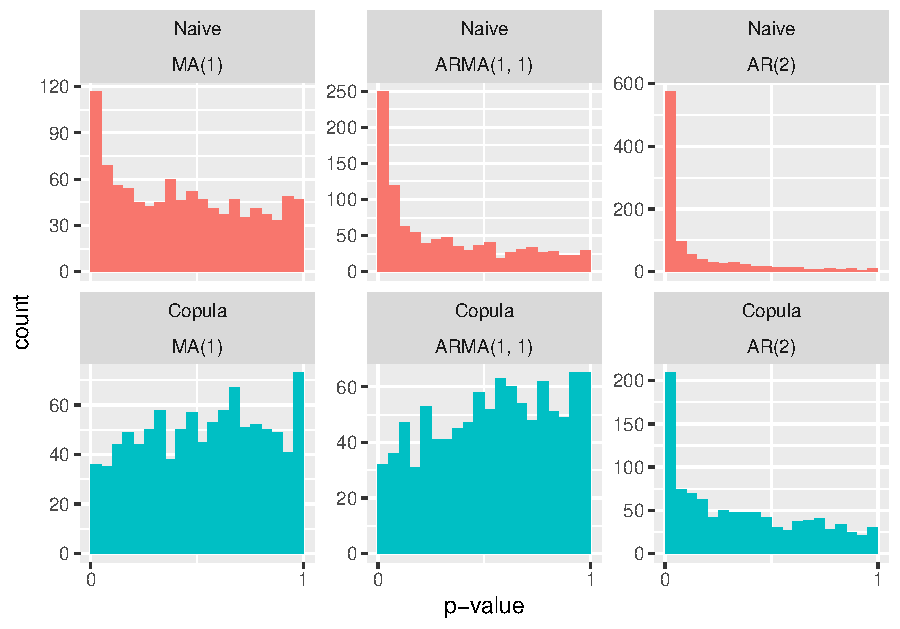
\includegraphics[width=\textwidth]{hist_ma1_arma_ar2_D}
  \caption{The Naive plots are the histograms of p-values from the standard KS
  test. The Copula plots are the histograms of p-values from parametric
  bootstrap with copulas for dependence. The data is generated from an MA(1)
  process (left) with $\theta = .5$, ARMA(1, 1) process (middle) with $\psi =
  .5$ and $\theta = .3$, and AR(2) process (right) with $\psi = (.5, .3)$ of the
  standard normal distribution. In each case, $1000$ replicate tests were
  performed with sample size $n = 100$ and $B = 1000$ bootstrap samples.}
  \label{fig:hist_ma1_arma_ar2_D}
\end{figure}

The procedure detailed in this section can also provide a reasonable
approximation in cases where the true dependence structure is not far from
AR(1). Figure~\ref{fig:hist_ma1_arma_ar2_D} shows the distribution of p-values
for dependence structures MA(1), ARMA(1, 1), and AR(2). As expected,
naively performing the KS test without correcting for dependence provides plots
of p-values that deviate from the uniform distribution. In the case of MA(1)
and ARMA(1, 1), the true dependence structure is close enough to our
assumption of AR(1) that the bootstrap procedure provides a reasonable
approximation. However, the AR(2) copula plot shows the limitation of this
technique as no AR(1) process can approximate an AR(2) process unless the
second-order coefficient is close to zero.

\begin{figure}[tbp]
  \centering
  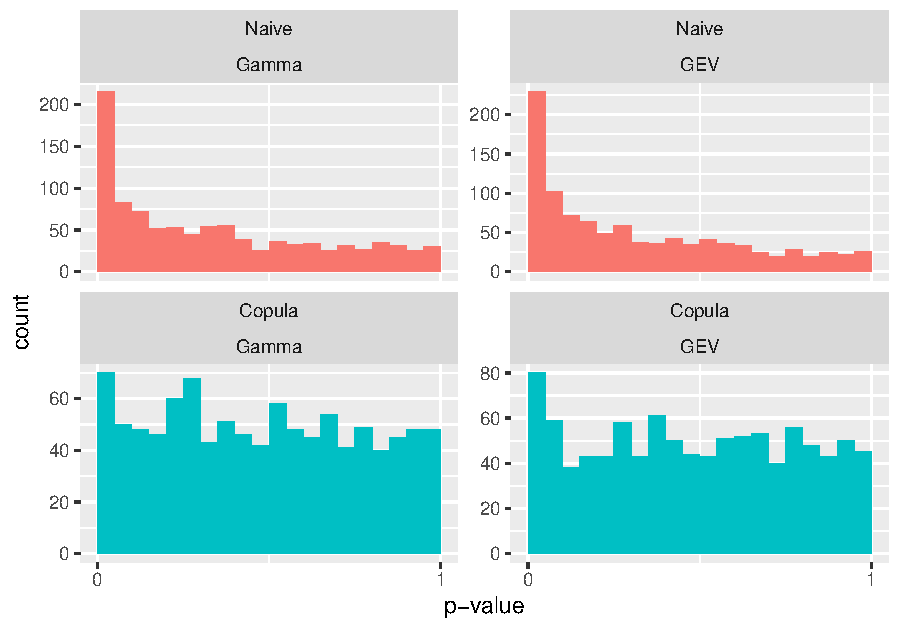
\includegraphics[width=\textwidth]{hist_gamma_gev_D}
  \caption{The Naive plots are the histograms of p-values from the standard KS
  test. The Copula plots are the histograms of p-values from parametric
  bootstrap with copulas for dependence. The data is generated from $Gamma(3,
  1)$ (left) and $GEV(0, .2, 1)$ (right) with a correlation coefficient of $r =
  0.5$. In each case, $1000$ replicate tests were performed with sample size $n
  = 100$ and $B = 1000$ bootstrap samples.}
  \label{fig:hist_gamma_gev_D}
\end{figure}

To further demonstrate the effectiveness of the procedure, we perform similar
simulations on other families of distributions.
Figure~\ref{fig:hist_gamma_gev_D} displays the results of tests using dependent
data generated from the gamma and the generalized extreme value distributions.
The procedure corrects the distribution of p-values for both distributions and
is shown to be applicable regardless of the family of distribution tested.


\section{Unspecified Parameters and Serially Dependent Data}
\label{sec:fittedwithdependence}

The procedure demonstrated in Section~\ref{sec:dependence} works when the data
is dependent and the hypothesized distribution is completely specified. However,
this is not practical. In practice we do not know the parameters of the
hypothesized distribution. Therefore, it is valuable to have a procedure that
corrects for both fitted parameters and serially dependent data. The remedy
using copulas can be modified to be effective in the case where both assumptions
must be violated. The null hypothesis is equivalent to Section~\ref{sec:fitted}
and the test statistic is equal to Equation~\eqref{eq:ks_fitted}. The bootstrap
procedure in Section~\ref{sec:fitted} is no longer valid because the serial
dependence is not accounted for. Let $r$ be the AR(1) coefficient of the normal
copula that matches the sample first-order Spearman's rho of the observed data
as obtained by the \texttt{iRho} function in the \textsf{copula} package
\citep{Copula}. We propose the following bootstrap procedure to assess the
significance of the observed KS statistic.

\begin{enumerate}
\item
  Generate $Z_1, \ldots, Z_n$ from an AR(1) process with autocorrelation
  coefficient $r$ such that the $Z_i$'s are $N(0, 1)$ variables.
\item
  Form a bootstrap sample $X_i^* = F^{-1}_{\hat\theta_n} [\Phi(Z_i)]$,
  $i = 1, \ldots, n$, whose first-order sample Spearman's rho matches that of
  the observed data.
\item
  Fit $F_\theta$ to the sample $X_1^*, \ldots, X_n^*$ and obtain estimator
  $\hat\theta_n^*$
\item
  Obtain the empirical distribution function $F_n^*$ of the bootstrap sample
  $X_1^*, \ldots, X_n^*$.
\item
  Calculate bootstrap KS statistic
  \[
    D^* = \sup_x \lvert F_n^* (x)- F_{\hat\theta_n^*}(x) \rvert.
  \]
\item
  Repeat the previous steps a large number $B$ times and use the empirical
    distribution of the $B$ test statistics to approximate
    the null distribution of the observed statistic.
\end{enumerate}

\begin{figure}[tbp]
  \centering
  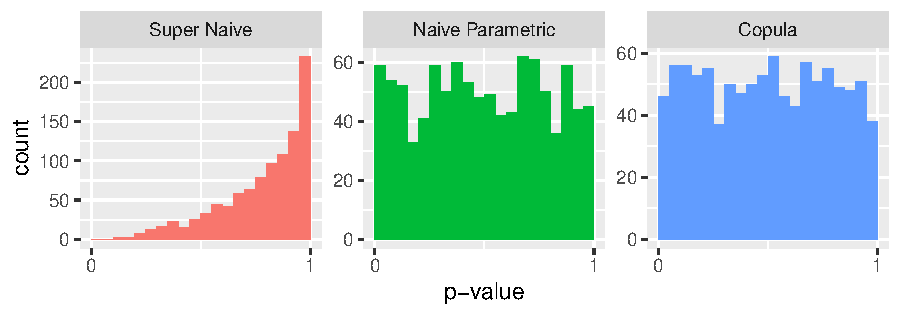
\includegraphics[width=\textwidth]{hist_ar1_FD}
  \caption{The Super Naive plot (left) is the histogram of p-values from the
  standard KS test with fitted parameters. The Naive Parametric plot (middle) is
  the histogram of p-values from implementing parametric bootstrap. The Copula
  plot is the histogram of p-values from implementing parametric bootstrap with
  copulas for dependence and correcting for fitted parameters. In each case,
  $1000$ replicate tests were performed with the data generated from an AR(1)
  process of the standard normal distribution with $\psi = .5$. The sample size
  is $n = 100$ and $B = 1000$ bootstrap samples are obtained for each test.}
  \label{fig:hist_ar1_FD}
\end{figure}

Figure~\ref{fig:hist_ar1_FD} shows the results of our simulation on data
simulated from an AR(1) process. As should be expected, naively fitting
parameters while providing no adjustment for dependent data invalidates the KS
test. As well, only using the parametric bootstrap remedy for fitted parameters
from Section~\ref{sec:fitted} seems to provide weaker results than the
copula remedy presented above. The results show that copula remedy generates
uniform p-values and restores the size of the KS test.

\begin{figure}[tbp]
  \centering
  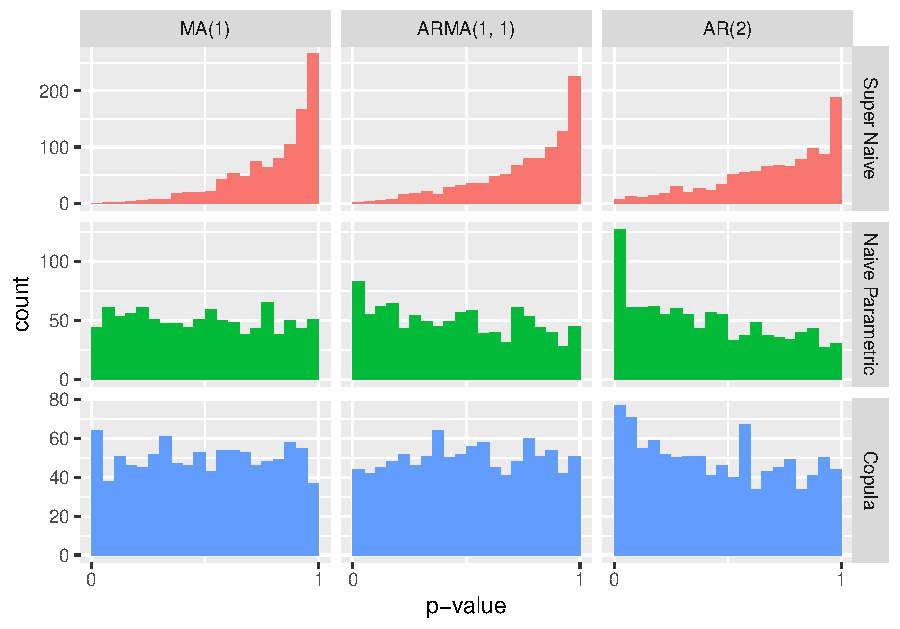
\includegraphics[width=\textwidth]{hist_ma1_arma_ar2_FD}
  \caption{The Super Naive plots (left) are the histograms of p-values from the
  standard KS test with fitted parameters. The Naive Parametric plots (middle)
  are the histograms of p-values from implementing parametric bootstrap. The
  Copula plots (bottom) are the histograms of p-values from implementing
  parametric bootstrap with copulas for dependence and correcting for fitted
  parameters. The data is generated from an MA(1) process (left) with
  $\theta = .5$, ARMA(1, 1) process (middle) with $\psi = .5$ and $\theta = .3$,
  and AR(2) process (right) with $\psi = (.5, .3)$ of the standard normal
  distribution. In each case, $1000$ replicate tests were performed with sample
  size $n = 100$ and $B = 1000$ bootstrap samples.}
  \label{fig:hist_ma1_arma_ar2_FD}
\end{figure}

Similar to Section~\ref{sec:dependence}, the copula approach is not a complete
solution. Regardless of the true dependence in the data we assume an AR(1)
dependence structure by taking the lag-1 sample auto-spearman rho. However, we
can show that as long as the AR(1) assumption is a close approximation, the
correction still provides a reasonable approximation that can be useful for
practical purposes. Figure~\ref{fig:hist_ma1_arma_ar2_FD} shows the results of the
procedure performed on data generated with dependence structures of  MA(1),
ARMA(1, 1), and AR(2). Naively fitting parameters and not adjusting for
dependence clearly deviates from a uniform distribution of p-values. Parametric
bootstrap provides some correction but does not account for dependence, so
therefore the results of the copula remedy are more accurate and favorable.
In the case of MA(1) and ARMA(1, 1), the true dependence appears close enough
to our assumption of AR(1) that the results are reasonable. AR(2) however
appears to be just far enough from our assumption, showing a limitation of the
procedure.

\begin{figure}[tbp]
  \centering
  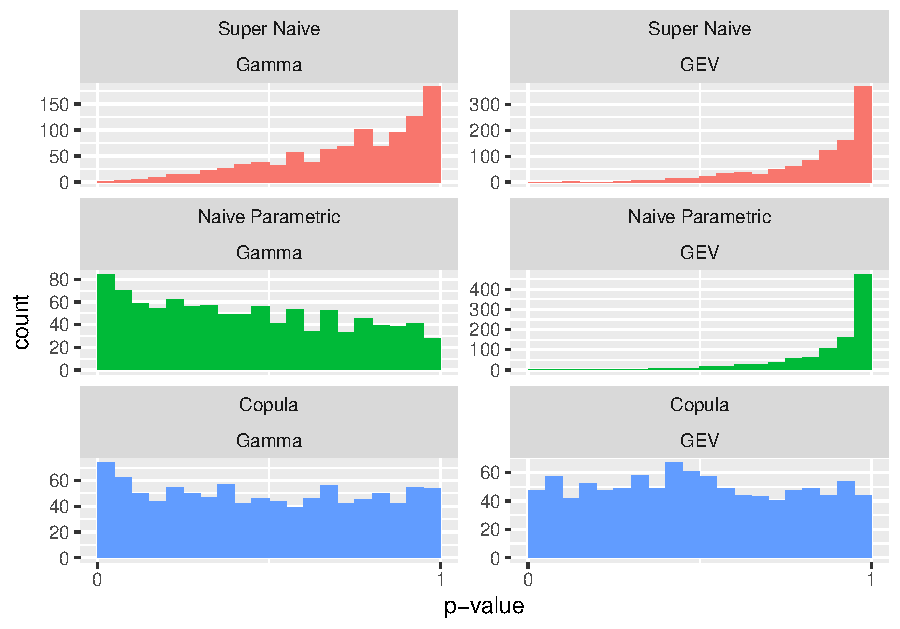
\includegraphics[width=\textwidth]{hist_gamma_gev_FD}
  \caption{The Super Naive plots (left) are the histograms of p-values from the
  standard KS test with fitted parameters. The Naive Parametric plots (middle)
  are the histograms of p-values from implementing parametric bootstrap. The
  Copula plots are the histograms of p-values from implementing parametric
  bootstrap with copulas for dependence and correcting for fitted parameters.
  The data is generated from $Gamma(3, 1)$ (left) and $GEV(0, .2, 1)$ (right)
  with a correlation coefficient of $r = 0.5$. In each case, $1000$ replicate
  tests were performed with sample size $n = 100$ and $B = 1000$ bootstrap
  samples.}
  \label{fig:hist_gamma_gev_FD}
\end{figure}

It is also possible to apply our procedure to other families of distributions.
The data in Figure~\ref{fig:hist_gamma_gev_FD} is generated from the gamma and
generalized extreme value distributions. The results are favorable and show that
the procedure outlined as a remedy for fitted parameters and spatially dependent
can be adapted for various families of distributions.


\section{Conclusion}
\label{sec:conclusion}

The KS test has base assumptions that the hypothesized distribution is
completely specified and the data is independent. When these assumptions are
violated, the test is no longer accurate and remedies must be performed. In the
case of fitted parameters, parametric and non-parametric bootstrap can restore
the size of the test. A bias correction is required if the non-parametric form
is used \citep{Babu}. In the case of \eds{serially} dependent data, a procedure
using bootstrap
with copulas to model dependency shows positive results. When both assumptions
are violated, i.e., where the data has \eds{serial} dependence and parameters
must
be fitted, an adjusted copula procedure also shows positive results. The tests
appear effective for a variety of families of distributions. The copula remedy
is not a complete solution and has limitations. Regardless of the true
dependence, we assume an AR(1) dependence structure. Therefore, if the AR(1)
dependence structure is a close approximation of the truth, the approach can work.
However, in cases such as AR(2), if the approximation is too far from the true
dependence structure the approach does not completely remedy the issue. As well,
tests were only performed with the normal copula. It is possible that other
copulas could provide stronger results based on the true dependence of the data.

\bibliographystyle{asa}
\bibliography{citations}


\end{document}
%%% LocalWords: 
%%% Local Variables:
%%% mode: latex
%%% TeX-master: t
%%% ispell-personal-dictionary: ".aspell.en.pws"
%%% fill-column: 80
%%% eval: (auto-fill-mode 1)
%%% End:
